\documentclass[aspectratio=169]{beamer} % Format widescreen 16:9 sesuai standar proyektor modern

\usepackage[utf8]{inputenc}
\usepackage{booktabs} % Untuk tabel yang rapi
\usepackage{graphicx} % Untuk memasukkan logo/gambar

\usepackage{tikz}
\usetikzlibrary{arrows.meta, positioning}

% ==========================================
% KUSTOMISASI WARNA RESMI ITS SURABAYA
% ==========================================
\definecolor{ITSBiruTua}{HTML}{243E80}   % Biru Cover ITS
\definecolor{ITSBiruMuda}{HTML}{007BC0}  % Biru Utama Lambang ITS
\definecolor{ITSKuning}{HTML}{FFF200}    % Kuning Lambang ITS
\definecolor{ITSAbuAbu}{HTML}{F0F4F8}    % Warna latar belakang box yang soft

% Menerapkan warna pada elemen-elemen Beamer
\setbeamercolor{structure}{fg=ITSBiruTua}
\setbeamercolor{palette primary}{bg=ITSBiruTua, fg=white}
\setbeamercolor{palette secondary}{bg=ITSBiruMuda, fg=white}
\setbeamercolor{palette tertiary}{bg=ITSBiruTua, fg=ITSKuning} % Judul utama menggunakan aksen kuning
\setbeamercolor{titlelike}{parent=palette primary, fg=white}

% Kustomisasi warna Blok/Kotak Informasi (Theorem, Block, dll)
\setbeamercolor{block title}{bg=ITSBiruTua, fg=white}
\setbeamercolor{block body}{bg=ITSAbuAbu, fg=black}

% Kustomisasi elemen teks & bullets
\setbeamercolor{item}{fg=ITSBiruMuda}
\setbeamercolor{subitem}{fg=ITSBiruTua}
\setbeamercolor{caption name}{fg=ITSBiruTua}

% ==========================================
% KUSTOMISASI TATA LETAK & FOOTER
% ==========================================
\usetheme{Madrid}
\usefonttheme[onlymath]{serif} % Font matematika tetap formal (serif)
\setbeamertemplate{navigation symbols}{} % Menghilangkan tombol navigasi kecil di kanan bawah

% Mengubah susunan footer agar menampilkan Nama Departemen/ITS
\setbeamertemplate{footline}{
	\leavevmode%
	\hbox{%
		\begin{beamercolorbox}[wd=.333333\paperwidth,ht=2.25ex,dp=1ex,center]{palette primary}%
			\usebeamerfont{author in head/foot}\insertshortauthor~~(ITS)
		\end{beamercolorbox}%
		\begin{beamercolorbox}[wd=.333333\paperwidth,ht=2.25ex,dp=1ex,center]{palette secondary}%
			\usebeamerfont{title in head/foot}\insertshorttitle
		\end{beamercolorbox}%
		\begin{beamercolorbox}[wd=.333333\paperwidth,ht=2.25ex,dp=1ex,right]{palette tertiary}%
			\usebeamerfont{date in head/foot}\insertshortdate{}\hspace*{2em}
			\insertframenumber{} / \inserttotalframenumber\hspace*{2ex} 
	\end{beamercolorbox}}%
	\vskip0pt%
}

% ==========================================
% METADATA DOSEN & MATAKULIAH
% ==========================================
\title[My Research Journey]{My Research Journey}
\subtitle{2010-2026}
\author[Dieky Adzkiya]{Dieky Adzkiya}
\institute[ITS]{
	Department of Mathematics \\
	Faculty of Science and Data Analytics \\
	Institut Teknologi Sepuluh Nopember
}
\date{\today}

% Otomatis menampilkan logo ITS kecil di kanan bawah setiap slide (opsional)
% Pastikan Anda sudah mengunggah file 'logo-its.png' di direktori project Overleaf Anda
\logo{
\includegraphics[height=0.6cm]{logo-its.png}}

% ==========================================
% OTOMATISASI DAFTAR ISI DI SETIAP AWAL SECTION
% ==========================================
\AtBeginSection[]
{
	\begin{frame}{Overview}
		\tableofcontents[currentsection]
	\end{frame}
}

% ==========================================
% MULAI DOKUMEN
% ==========================================
\begin{document}
	
	% 1. Slide Judul (Title Page)
	\begin{frame}
		\titlepage
	\end{frame}
	
	% 2. Slide Daftar Isi (Table of Contents)
	\begin{frame}{Overview}
		\tableofcontents
	\end{frame}
	
	\section{Finite Abstractions of Max-Plus-Linear Systems}
	% 3. Slide Konten Standard (Poin-poin)
	\begin{frame}{Background}{Formal Verification and Model Checking}
		Formal verification is a mathematical method used to prove that a model satisfies a specification under \textbf{all possible conditions}:
		\begin{itemize}
			\item model checking
			\item theorem proving (deductive verification)
			\item equivalence checking
		\end{itemize}
		
		\-\\
		
		Model checking is \textbf{an automated formal verification technique} that exhaustively explores all possible states of a system to mathematically prove it meets specified properties:
		\begin{itemize}
			\item fully automated
			\item finite state
		\end{itemize}
		
		\-\\
		
		Since Max-Plus-Linear (MPL) systems have infinitely many states, ...
	\end{frame}
	
	\begin{frame}{Abstraction}
		
		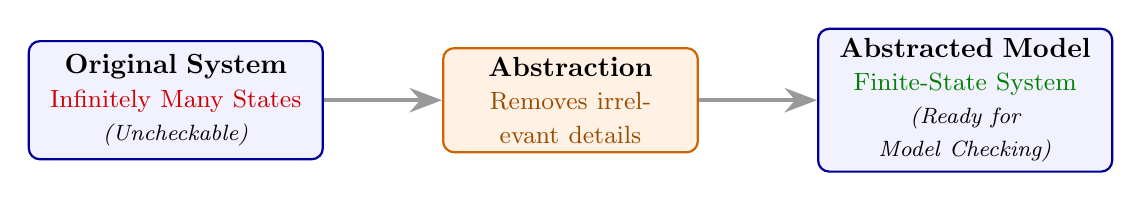
\begin{tikzpicture}[
			% Gaya untuk kotak proses (Node Styles)
			block/.style={
				rectangle, 
				draw=blue!60!black, 
				fill=blue!5, 
				thick, 
				text width=3.5cm, 
				align=center, 
				minimum height=1.5cm, 
				rounded corners
			},
			process/.style={
				rectangle, 
				draw=orange!80!black, 
				fill=orange!10, 
				thick, 
				text width=3cm, 
				align=center, 
				minimum height=1.2cm, 
				rounded corners
			},
			% Gaya untuk garis panah
			arrow/.style={
				-{Stealth[scale=1.2]}, 
				thick, 
				draw=gray!80,
				line width=1.5pt
			}
			]
			
			% Menempatkan komponen-komponen (Nodes)
			\node[block] (infinite) {
				\textbf{Original System}\\
				\textcolor{red!80!black}{\small Infinitely Many States}\\
				\textit{\footnotesize (Uncheckable)}
			};
			
			\node[process, right=1.5cm of infinite] (abstraction) {
				\textbf{Abstraction}\\
				\small \textcolor{orange!60!black}{Removes irrelevant details}
			};
			
			\node[block, right=1.5cm of abstraction] (finite) {
				\textbf{Abstracted Model}\\
				\textcolor{green!50!black}{\small Finite-State System}\\
				\textit{\footnotesize (Ready for Model Checking)}
			};
			
			% Menghubungkan komponen dengan panah
			\draw[arrow] (infinite) -- (abstraction);
			\draw[arrow] (abstraction) -- (finite);
			
		\end{tikzpicture}
		
		\-\\
		
		The solution: abstraction
		\begin{itemize}
			\item simplifies a complex or infinite system by removing irrelevant details
			\item transforms an infinite-state system into a manageable finite-state model
		\end{itemize}
		
		\-\\
		
		The relationship between the abstracted model and the original system is ...
		
	\end{frame}
	
	\begin{frame}{Property Preservation in Abstraction}
		
		The abstracted model:
		\begin{itemize}
			\item \textbf{simulates} the original system
			\item contains \textbf{more} behaviors than the original system 
		\end{itemize}
		
		\-\\
		
		Scenario 1: The property holds true
		\begin{itemize}
			\item \textbf{Observation} A linear-time property is satisfied by the abstracted system
			\item \textbf{Conclusion} The original system is guaranteed to satisfy the property
			\item \textbf{Why} If the larger, looser model is safe, the smaller, stricter original model must be safe
		\end{itemize}
		
		\-\\
		
		Scenario 2: The property fails
		\begin{itemize}
			\item \textbf{Observation} A linear-time property is violated by the abstracted system
			\item \textbf{Conclusion} The original system might still satisfy the property
			\item \textbf{Why} The failure could be a spurious counterexample (a false alarm caused by a behavior that only exists in the abstracted model, not in the original system)
		\end{itemize}
		
	\end{frame}
	
	\begin{frame}{Problem Formulation and Proposed Solution}
		
		Problem formulation:
		\begin{itemize}
			\item Formal verification (specifically, model checking) of MPL systems
			
			\item Finite abstractions of MPL systems
		\end{itemize}
		
		\-\\
		
		\begin{block}{}
			Formal verification is a mathematical method used to prove that \textbf{a model} satisfies \textbf{a specification} under all possible conditions
		\end{block}
		
		\-\\
		
		\begin{itemize}
			\item Model: MPL systems
			\item Specification: Linear Temporal Logic (LTL) is classified as a linear-time property
		\end{itemize}
		
		\-\\
		
		Proposed solution: abstraction of MPL systems
		\begin{enumerate}
			\item Partitioning the state space
			\item Computing the transition relation
		\end{enumerate}
		
	\end{frame}
	
	\begin{frame}{Linear Temporal Logic (LTL)}
		
		LTL is a formal language used to express properties and requirements of a system over time
		
		\-\\
		
		\begin{block}{Core temporal operators}
		\begin{tabular}{ll}
			Always $\Box$ & the condition must hold true at every state in the future \\[1ex]
			Eventually $\Diamond$ & the condition will become true at some point in the future \\[1ex]
			Next $\bigcirc$ & the condition must be true in the very next state \\[1ex]
			Until $\mathbf{U}$ & condition A must remain true until condition B becomes true \\[1ex]
		\end{tabular}
		\end{block}
		
		\-\\
		
		\begin{itemize}
			\item In railway network, let $x_i(k)$ represents the $k$-th departure time of station $i$
			
			\item The LTL $\Box (x_i(k) - x_j(k) \leq 5)$ is equivalent with ``$x_i(k) - x_j(k) \leq 5$ for all $k \in \{0,1,\dots\}$''
			
			\item The difference of departure time between station $i$ and station $j$ is at most 5 minutes
		\end{itemize}
		
	\end{frame}
	
	\begin{frame}{References}
		
		Adzkiya, D., De Schutter, B., \& Abate, A. (2013). Finite abstractions of max-plus-linear systems. \textit{IEEE Transactions on Automatic Control}, 58(12), 3039-3053.
		
		\-\\
		
		Soudjani, S. E. Z., Adzkiya, D., \& Abate, A. (2015). Formal verification of stochastic max-plus-linear systems. \textit{IEEE Transactions on Automatic Control}, 61(10), 2861-2876.
		
		\-\\
		
		Adzkiya, D., Zhang, Y., \& Abate, A. (2016). VeriSiMPL 2: An open-source software for the verification of max-plus-linear systems. \textit{Discrete Event Dynamic Systems}, 26(1), 109-145.
		
	\end{frame}
	
	\section{Reachability of Max-Plus-Linear Systems}
	
	\begin{frame}{Forward Reachability Analysis}
		
		\begin{block}{Reach set}
			Given an MPL system and a nonempty set of initial conditions $X_0 \subseteq \mathbb{R}^n$, the reach set $X_N$ at the event step $N > 0$ is the set of all states $\{ x(N) : x(0) \in X_0 \}$ obtained via the MPL dynamics.
		\end{block}
		
		\-\\
		
		\begin{block}{Reach tube}
			Given an MPL system and a nonempty set of initial conditions $X_0 \subseteq \mathbb{R}^n$, the reach tube is defined by the set-valued function $k \mapsto X_k$ for any given $k > 0$ where $X_k$ is defined.
		\end{block}
		
		\-\\
		
		If the difference of initial departure between station $i$ and station $j$ is at most 5 minutes, i.e.\ $x_i(0) - x_j(0) \leq 5$, what is their difference in the 10th departure, i.e.\ $x_i(9) - x_j(9)$?
		
	\end{frame}
	
	\begin{frame}{Backward Reachability Analysis}
		
		\begin{block}{Backward reach set}
			Given an MPL system and a nonempty set of final conditions $X_0 \subseteq \mathbb{R}^n$, the backward reach set $X_{-N}$ is the set of all states $x(-N)$ that lead to $X_0$ in $N$ steps of the MPL dynamics.
		\end{block}
		
		\-\\
		
		\begin{block}{Backward reach tube}
			Given an MPL system and a nonempty set of final conditions $X_0 \subseteq \mathbb{R}^n$, the backward reach tube is defined by the set-valued function $k \mapsto X_{-k}$ for any given $k > 0$ where $X_{-k}$ is defined.
		\end{block}
		
		\-\\
		
		If the difference of 10th departure between station $i$ and station $j$ is at most 5 minutes, i.e.\ $x_i(9) - x_j(9) \leq 5$, what is their difference in the initial departure, i.e.\ $x_i(0) - x_j(0)$?
		
	\end{frame}
	
	\begin{frame}{References}
		
		Adzkiya, D., De Schutter, B., \& Abate, A. (2015). Computational techniques for reachability analysis of max-plus-linear systems. Automatica, 53, 293-302.
		
		\-\\
		
		Mufid, M. S., Adzkiya, D., \& Abate, A. (2020). Symbolic reachability analysis of high dimensional max-plus linear systems. IFAC-PapersOnLine, 53(4), 459-465.
		
		\-\\
		
		Mufid, M. S., Adzkiya, D., \& Abate, A. (2021). SMT-based reachability analysis of high dimensional interval max-plus linear systems. IEEE Transactions on Automatic Control, 67(6), 2700-2714.
		
	\end{frame}
	
	\section{Control Design of Autonomous Vehicles using Satisfiability Modulo Theory}
	
	\begin{frame}{Satisfiability Modulo Theory}
		
		Satisfiability Modulo Theories (SMT) is the problem of determining whether a mathematical formula is satisfiable
		\begin{align*}
			(\mathtt{x} \geq 0) \wedge (\mathtt{y} < 2) \wedge (\mathtt{x} - \mathtt{y} < -1)
		\end{align*}
		has solution (\textbf{satisfiable}) if variables are reals (e.g.\ $\mathtt{x} = 0.1$ and $\mathtt{y} = 1.2$) \\
		no solution (\textbf{unsatisfiable}) if variables are integers
		
		\begin{block}{SMT Solver}
			\begin{itemize}
				\item \textbf{Definition} An SMT Solver is a software tool that checks whether an SMT problem is satisfiable.
				\item \textbf{Output} If the problem is satisfiable, the solver provides a concrete satisfying model (example).
				\item \textbf{Popular Examples} Z3 (Microsoft Research), cvc5 (Stanford/Iowa), and Yices2 (SRI).
			\end{itemize}
		\end{block}
		
	\end{frame}
	
	\begin{frame}{The Proposed Method}
		
		\begin{enumerate}
			\item Discretize the model using a finite difference scheme
			\item Construct the SMT
			\begin{itemize}
				\item initial position
				\item final position
				\item road position
				\item dynamical system
			\end{itemize}
			\item Solve the SMT problem
			\begin{itemize}
				\item if satisfiable, the solution is the controller
				\item if unsatisfiable, analyze the possible causes and update the SMT accordingly
			\end{itemize}
		\end{enumerate}
		
	\end{frame}
	
	\begin{frame}{References}
		
		Adzkiya, D., Mufid, M. S., Saputri, F. S., \& Abate, A. (2024). Control design of discrete-time unicycle model using satisfiability modulo theory. Systems Science \& Control Engineering, 12(1), 2316166.
		
	\end{frame}
	
	\section{Future Plan}
	
	\begin{frame}{Future Plan}
	
	\begin{itemize}
		\item PHC Nusantara and beyond
		\item Department of Mathematics: joint research, double degree, student exchange, \dots
		\item Collaboration between research centers
	\end{itemize}
	
	\vfill
	
	\begin{center}
		\Large\bfseries\color{ITSBiruTua} Thank You \\
		\vspace{0.3cm}
		\large\color{ITSBiruMuda} Any Questions?
	\end{center}
		
	\end{frame}
	
\end{document}
